\documentclass[12pt, a4paper]{article}

% ----- Mandatory Packages -----
\usepackage{amsmath}
\usepackage{amssymb}
\usepackage{amsthm}
\usepackage{geometry}
\usepackage{tikz}
\usetikzlibrary{arrows.meta, positioning, shapes, calc, trees}
\usepackage{mathrsfs}
\usepackage{mathtools}
\usepackage{xcolor}
\usepackage{enumitem}
\usepackage{hyperref}

% ----- Page Geometry -----
\geometry{
    top=1in,
    bottom=1in,
    left=1in,
    right=1in
}

% ----- Theorem Environments -----
\newtheorem{theorem}{Theorem}[section]
\newtheorem{lemma}[theorem]{Lemma}
\newtheorem{proposition}[theorem]{Proposition}
\newtheorem{corollary}[theorem]{Corollary}
\theoremstyle{definition}
\newtheorem{definition}{Definition}[section]
\newtheorem{axiom}{Axiom}[section]
\newtheorem{example}{Example}[section]
\theoremstyle{remark}
\newtheorem{remark}{Remark}[section]

% ----- Custom Commands -----
\newcommand{\R}{\mathbb{R}}
\newcommand{\E}{\mathbb{E}}
\newcommand{\Prob}{\mathbb{P}}
\newcommand{\F}{\mathcal{F}}
\newcommand{\G}{\mathcal{G}}
\newcommand{\W}{\Omega}
\newcommand{\1}{\mathbf{1}}
\DeclarePairedDelimiter{\abs}{\lvert}{\rvert}

% ----- Document Meta -----
\title{\textbf{Homework 2 \\ Advanced Probability, Conditioning, and Measure-Theoretic Foundations}}
\author{Tashfeen Omran}
\date{September 2026}

\begin{document}

\maketitle
\tableofcontents
\newpage

% ==========================================
% PART 1: Comprehensive Introduction
% ==========================================
\section{Part 1: Comprehensive Introduction, Context, and Prerequisites}

\subsection{Historical Context and Motivation}
Historically, probability was conceptualized through the lens of gambling and discrete combinatorial games, formalized by mathematicians like Blaise Pascal and Pierre de Fermat in the 17th century. However, as probability began integrating with continuous calculus and real-world statistical physics, fundamental paradoxes emerged (such as Bertrand's Paradox). The mathematical community faced a foundational crisis: what \textit{is} a probability, strictly speaking? In 1933, Andrey Kolmogorov provided the definitive resolution by embedding probability theory within the rigorous framework of abstract measure theory. By defining a sample space, a $\sigma$-algebra of events, and a normalized measure, Kolmogorov eliminated intuitive ambiguities, making advanced constructs like conditional expectation and stochastic processes logically sound. 

\subsection{Core Concepts, Axioms, and Foundations}
To treat probability with the rigor of abstract mathematics, we must abandon intuitive notions of "chance" and replace them with precise set-theoretic constructs. We define a \textbf{Probability Space} as a triplet $(\W, \F, \Prob)$:
\begin{itemize}
    \item \textbf{Sample Space ($\W$):} A non-empty set containing all possible outcomes of an experiment. Each $\omega \in \W$ is a sample point.
    \item \textbf{$\sigma$-algebra ($\F$):} A collection of subsets of $\W$ representing "measurable events." $\F$ must satisfy three properties: (1) $\W \in \F$, (2) if $A \in \F$, then its complement $A^c \in \F$, and (3) if $A_1, A_2, \dots \in \F$, then their countable union $\bigcup_{i=1}^\infty A_i \in \F$.
    \item \textbf{Probability Measure ($\Prob$):} A set function $\Prob: \F \to [0, 1]$ satisfying Kolmogorov's Axioms.
\end{itemize}

\begin{axiom}[Kolmogorov's Axioms]
\label{ax:kolmogorov}
The measure $\Prob$ must satisfy:
\begin{enumerate}
    \item \textbf{Non-negativity:} $\Prob(A) \ge 0$ for all $A \in \F$.
    \item \textbf{Unit Measure:} $\Prob(\W) = 1$.
    \item \textbf{Countable Additivity:} If $A_1, A_2, \dots \in \F$ are mutually exclusive (i.e., $A_i \cap A_j = \emptyset$ for $i \neq j$), then $\Prob\left(\bigcup_{i=1}^\infty A_i\right) = \sum_{i=1}^\infty \Prob(A_i)$.
\end{enumerate}
\end{axiom}

From this foundation, we construct \textbf{Conditional Probability}. The quantity $\Prob(A|B)$ intuitively restricts our universe $\W$ to the subset $B$. Mathematically, conditioning on an event $B$ (where $\Prob(B) > 0$) induces a \textit{new} probability measure $\Prob_B(\cdot) = \Prob(\cdot \cap B) / \Prob(B)$ on the measurable space $(\W, \F)$.

\subsection{Key Theorems, Lemmas, and Formulas}
\begin{theorem}[Multiplicative Law of Probability]
For any two events $A, B \in \F$, 
\[ \Prob(A \cap B) = \Prob(A) \Prob(B|A) = \Prob(B) \Prob(A|B) \]
For mutually independent events, this reduces to $\Prob(A \cap B) = \Prob(A)\Prob(B)$.
\end{theorem}

\begin{theorem}[Additive Law of Probability (Inclusion-Exclusion)]
For any two events $A, B \in \F$,
\[ \Prob(A \cup B) = \Prob(A) + \Prob(B) - \Prob(A \cap B) \]
\end{theorem}

\begin{theorem}[Law of Total Probability]
\label{thm:ltp}
Let $\{B_1, B_2, \dots, B_k\}$ be a partition of the sample space $\W$ (i.e., mutually disjoint and $\bigcup_{i=1}^k B_i = \W$), such that $\Prob(B_i) > 0$ for all $i$. Then for any event $A \in \F$:
\[ \Prob(A) = \sum_{i=1}^k \Prob(A \cap B_i) = \sum_{i=1}^k \Prob(A | B_i)\Prob(B_i) \]
\end{theorem}

\begin{theorem}[Bayes' Rule]
Under the same partition conditions as Theorem \ref{thm:ltp}, the conditional probability of a partition element $B_j$ given event $A$ (where $\Prob(A) > 0$) is:
\[ \Prob(B_j | A) = \frac{\Prob(A | B_j)\Prob(B_j)}{\sum_{i=1}^k \Prob(A | B_i)\Prob(B_i)} \]
\end{theorem}

\subsection{Prerequisites}
Mastery of this chapter requires:
\begin{enumerate}
    \item \textbf{Naive Set Theory:} Fluency in unions ($\cup$), intersections ($\cap$), complements ($\bar{A}$ or $A^c$), subsets ($\subset$), and partitions.
    \item \textbf{Logical Equivalences:} Mastery of De Morgan's Laws: $\overline{A \cup B} = \bar{A} \cap \bar{B}$ and $\overline{A \cap B} = \bar{A} \cup \bar{B}$.
    \item \textbf{Algebraic Manipulation:} Ability to iteratively solve systems of linear probabilistic equalities.
    \item \textbf{Combinatorics:} Understanding of combinations, permutations, and factorials to establish cardinalities of discrete sample spaces.
\end{enumerate}

\newpage

% ==========================================
% PART 2: Detailed Homework Solutions
% ==========================================
\section{Part 2: Detailed Homework Solutions (Rigorous Proofs \& Computations)}
\textit{Note: All examples provided in the Chapter 2 assignment are rigorously proven below. The notation $\bar{A}$ and $A^c$ are used interchangeably for the complement of $A$.}

% --- Example 1 ---
\subsection*{Example 1: Conditional Probabilities on a Die}
\begin{proof}[Solution to Example 1]
\textbf{Setup:} Let $\W = \{1, 2, 3, 4, 5, 6\}$ be the sample space of a single toss of a balanced discrete uniform 6-sided die. The $\sigma$-algebra is the power set $\F = 2^\W$, and the measure is defined by $\Prob(\{\omega\}) = 1/6$ for all $\omega \in \W$. 
Let event $A$ = \{Observe a 1\} = $\{1\}$, and event $B$ = \{Observe an odd number\} = $\{1, 3, 5\}$.
We are asked to find specific probabilities.

\textbf{Step 1: Compute basic measures and intersections.}
$\Prob(A) = \frac{\abs{A}}{\abs{\W}} = \frac{1}{6}$.
$\Prob(B) = \frac{\abs{B}}{\abs{\W}} = \frac{3}{6} = \frac{1}{2}$.
The intersection $A \cap B = \{1\} \cap \{1, 3, 5\} = \{1\}$. Thus, $\Prob(A \cap B) = \frac{1}{6}$.
The union $A \cup B = \{1\} \cup \{1, 3, 5\} = \{1, 3, 5\} = B$.

\textbf{Step 2: Solve sub-problems using conditional probability definitions.}
\begin{itemize}[leftmargin=*]
    \item \textbf{(a) Find $\Prob(A|B)$:} 
    By definition, $\Prob(A|B) = \frac{\Prob(A \cap B)}{\Prob(B)} = \frac{1/6}{3/6} = \frac{1}{3}$. 
    \textit{Conclusion:} $\Prob(A|B) = 1/3$.
    
    \item \textbf{(b) Find $\Prob(B|A)$:}
    By definition, $\Prob(B|A) = \frac{\Prob(A \cap B)}{\Prob(A)} = \frac{1/6}{1/6} = 1$. 
    \textit{Conclusion:} $\Prob(B|A) = 1$.
    
    \item \textbf{(c) Find $\Prob(A | A \cup B)$:}
    Since $A \cup B = B$, we substitute directly: $\Prob(A | A \cup B) = \Prob(A | B)$. From part (a), this is $1/3$.
    Alternatively, using definitions: $\Prob(A | A \cup B) = \frac{\Prob(A \cap (A \cup B))}{\Prob(A \cup B)}$. By absorption laws of sets, $A \cap (A \cup B) = A$. 
    Thus, $\frac{\Prob(A)}{\Prob(A \cup B)} = \frac{1/6}{3/6} = \frac{1}{3}$.
    
    \item \textbf{(d) Find $\Prob(A \cap B | A \cup B)$:}
    By definition, $\frac{\Prob((A \cap B) \cap (A \cup B))}{\Prob(A \cup B)}$. Since $(A \cap B) \subset (A \cup B)$, the intersection simplifies to $A \cap B$. 
    Thus, $\frac{\Prob(A \cap B)}{\Prob(A \cup B)} = \frac{1/6}{3/6} = \frac{1}{3}$.
\end{itemize}
This completes the rigorous evaluation of Example 1.
\end{proof}

% --- Example 2 ---
\subsection*{Example 2: Abstract Event Conditional Logic}
\begin{proof}[Solution to Example 2]
\textbf{Setup:} We are given an abstract probability space containing events $A$ and $B$. We are given the following measures: $\Prob(A) = 0.5$, $\Prob(B) = 0.3$, $\Prob(A \cap B) = 0.1$, and $\Prob(A \cup B) = 0.7$. 
(Note: By the Additive Law, $\Prob(A \cup B) = 0.5 + 0.3 - 0.1 = 0.7$, so the given system is mathematically consistent).

\begin{itemize}[leftmargin=*]
    \item \textbf{(a) $\Prob(A|B)$:} $\frac{\Prob(A \cap B)}{\Prob(B)} = \frac{0.1}{0.3} = \frac{1}{3}$.
    \item \textbf{(b) $\Prob(B|A)$:} $\frac{\Prob(A \cap B)}{\Prob(A)} = \frac{0.1}{0.5} = \frac{1}{5}$.
    \item \textbf{(c) $\Prob(A | A \cup B)$:} $\frac{\Prob(A \cap (A \cup B))}{\Prob(A \cup B)} = \frac{\Prob(A)}{\Prob(A \cup B)} = \frac{0.5}{0.7} = \frac{5}{7}$.
    \item \textbf{(d) $\Prob(A | A \cap B)$:} $\frac{\Prob(A \cap (A \cap B))}{\Prob(A \cap B)} = \frac{\Prob(A \cap B)}{\Prob(A \cap B)} = 1$. (Given the intersection occurs, $A$ has trivially occurred).
    \item \textbf{(e) $\Prob(A \cap B | A \cup B)$:} $\frac{\Prob((A \cap B) \cap (A \cup B))}{\Prob(A \cup B)} = \frac{\Prob(A \cap B)}{\Prob(A \cup B)} = \frac{0.1}{0.7} = \frac{1}{7}$.
\end{itemize}
Computations match the desired arithmetic properties of probability measures.
\end{proof}

% --- Example 3 ---
\subsection*{Example 3: Independence Checking}
\begin{proof}[Solution to Example 3]
\textbf{Setup:} $\W = \{1,2,3,4,5,6\}$ with uniform probability. Define events $A = \{1,3,5\}$ (Odd), $B = \{2,4,6\}$ (Even), and $C = \{1,2\}$ (1 or 2). We compute prior probabilities:
$\Prob(A) = 3/6 = 1/2$. $\Prob(B) = 3/6 = 1/2$. $\Prob(C) = 2/6 = 1/3$.

\textbf{(a) Are $A$ and $B independent?$}
By definition, events are independent iff $\Prob(A \cap B) = \Prob(A)\Prob(B)$.
Observe that $A \cap B = \emptyset \implies \Prob(A \cap B) = 0$.
However, $\Prob(A)\Prob(B) = (1/2)(1/2) = 1/4$.
Since $0 \neq 1/4$, $A$ and $B$ are \textbf{dependent}. \textit{Note: Non-empty mutually exclusive events are always dependent.}

\textbf{(b) Are $A$ and $C independent?$}
Intersection $A \cap C = \{1,3,5\} \cap \{1,2\} = \{1\} \implies \Prob(A \cap C) = 1/6$.
Compute the product of marginals: $\Prob(A)\Prob(C) = (1/2)(1/3) = 1/6$.
Since $\Prob(A \cap C) = \Prob(A)\Prob(C)$, events $A$ and $C$ are mathematically \textbf{independent}.
\end{proof}

% --- Example 4 ---
\subsection*{Example 4: Survey Independence (Empirical Measure)}
\begin{proof}[Solution to Example 4]
\textbf{Setup:} We are provided a contingency matrix mapping a sample space of 100 adults. Let $D$ be "Yes Child in College", $E$ be "No Child", $A$ be "Too High", $B$ be "About Right", $C$ be "Too Little". From the table margins:
$\Prob(A) = 0.61$, $\Prob(B) = 0.30$, $\Prob(C) = 0.09$, and $\Prob(D) = 0.30$. 
The joint probabilities are the internal cells, e.g., $\Prob(A \cap D) = 0.20$.

We must verify independence by checking if $\Prob(X | Y) = \Prob(X)$, or equivalently, $\Prob(X \cap Y) = \Prob(X)\Prob(Y)$.

\textbf{(a) $A$ and $D independent?$}
$\Prob(A|D) = \frac{\Prob(A \cap D)}{\Prob(D)} = \frac{0.20}{0.30} \approx 0.667$.
Since $\Prob(A|D) = 0.667 \neq 0.61 = \Prob(A)$, $A$ and $D$ are \textbf{dependent}.

\textbf{(b) $B$ and $D independent?$}
$\Prob(B|D) = \frac{\Prob(B \cap D)}{\Prob(D)} = \frac{0.09}{0.30} = 0.30$.
Since $\Prob(B|D) = 0.30 = \Prob(B)$, $B$ and $D$ are \textbf{independent}.

\textbf{(c) $C$ and $D independent?$}
$\Prob(C|D) = \frac{\Prob(C \cap D)}{\Prob(D)} = \frac{0.01}{0.30} \approx 0.033$.
Since $\Prob(C|D) \approx 0.033 \neq 0.09 = \Prob(C)$, $C$ and $D$ are \textbf{dependent}.
\end{proof}

% --- Example 5 ---
\subsection*{Example 5: Laws of Probability with Complements}
\begin{proof}[Solution to Example 5]
\textbf{Setup:} We are given $\Prob(A) = 0.2$, $\Prob(B) = 0.3$, and $\Prob(A \cup B) = 0.4$.

\textbf{(a) Find $\Prob(A \cap B)$:}
Using the Additive Law: $\Prob(A \cup B) = \Prob(A) + \Prob(B) - \Prob(A \cap B)$.
$0.4 = 0.2 + 0.3 - \Prob(A \cap B) \implies \Prob(A \cap B) = 0.5 - 0.4 = 0.1$.

\textbf{(b) Find $\Prob(\bar{A} \cup \bar{B})$:}
Using De Morgan's Law, $\bar{A} \cup \bar{B} = \overline{A \cap B}$.
Thus, $\Prob(\bar{A} \cup \bar{B}) = 1 - \Prob(A \cap B) = 1 - 0.1 = 0.9$.

\textbf{(c) Find $\Prob(\bar{A} \cap \bar{B})$:}
Using De Morgan's Law, $\bar{A} \cap \bar{B} = \overline{A \cup B}$.
Thus, $\Prob(\bar{A} \cap \bar{B}) = 1 - \Prob(A \cup B) = 1 - 0.4 = 0.6$.

\textbf{(d) Find $\Prob(\bar{A} | B)$:}
By definition, $\Prob(\bar{A} | B) = \frac{\Prob(\bar{A} \cap B)}{\Prob(B)}$.
Notice that $B = (A \cap B) \cup (\bar{A} \cap B)$, which are mutually exclusive.
Thus, $\Prob(B) = \Prob(A \cap B) + \Prob(\bar{A} \cap B) \implies \Prob(\bar{A} \cap B) = \Prob(B) - \Prob(A \cap B)$.
$\Prob(\bar{A} \cap B) = 0.3 - 0.1 = 0.2$.
Therefore, $\Prob(\bar{A} | B) = \frac{0.2}{0.3} = \frac{2}{3} \approx 0.667$.
\end{proof}

% --- Example 6 ---
\subsection*{Example 6: Evaluating Events under Strict Independence}
\begin{proof}[Solution to Example 6]
\textbf{Setup:} $A$ and $B$ are independent. $\Prob(A) = 0.5, \Prob(B) = 0.2$. Independence implies $\Prob(A \cap B) = \Prob(A)\Prob(B) = (0.5)(0.2) = 0.1$.

\textbf{(a) $\Prob(A \cup B)$:} 
By the Additive Law: $\Prob(A \cup B) = \Prob(A) + \Prob(B) - \Prob(A \cap B) = 0.5 + 0.2 - 0.1 = 0.6$.

\textbf{(b) $\Prob(\bar{A} \cup \bar{B})$:} 
By De Morgan's: $\Prob(\overline{A \cap B}) = 1 - \Prob(A \cap B) = 1 - 0.1 = 0.9$.

\textbf{(c) $\Prob(\bar{A} \cap \bar{B})$:} 
By De Morgan's: $\Prob(\overline{A \cup B}) = 1 - \Prob(A \cup B) = 1 - 0.6 = 0.4$.
\textit{Alternative verification:} Since $A, B$ independent, $\bar{A}, \bar{B}$ are independent. $\Prob(\bar{A})\Prob(\bar{B}) = (1-0.5)(1-0.2) = (0.5)(0.8) = 0.4$.
\end{proof}

% --- Example 7 ---
\subsection*{Example 7: Event Composition and the Complement Rule}
\begin{proof}[Solution to Example 7]
\textbf{Setup:} A patient responds to treatment with $p=0.9$. Let $B_i$ be the event the $i$-th patient responds. The events $\{B_1, B_2, B_3\}$ are mutually independent. We wish to find $A = \text{at least 1 responds} = B_1 \cup B_2 \cup B_3$.

\textbf{Strategy: Complement space manipulation.} 
Direct calculation of the union of 3 events is tedious. We evaluate the complement $\bar{A}$, which is the event that \textit{none} of the 3 patients respond.
$\bar{A} = \bar{B}_1 \cap \bar{B}_2 \cap \bar{B}_3$.
Because $B_i$ are independent, their complements $\bar{B}_i$ are independent.
$\Prob(\bar{A}) = \Prob(\bar{B}_1)\Prob(\bar{B}_2)\Prob(\bar{B}_3) = (1-0.9)(1-0.9)(1-0.9) = (0.1)^3 = 0.001$.
Finally, $\Prob(A) = 1 - \Prob(\bar{A}) = 1 - 0.001 = 0.999$.
\end{proof}

% --- Example 8 ---
\subsection*{Example 8: Combinatorics and Inclusion-Exclusion}
\begin{proof}[Solution to Example 8]
\textbf{Setup:} A monkey tosses one red, one black, and one white ball randomly into 3 corresponding boxes. 
Sample Space $\W$ consists of all permutations of 3 balls into 3 boxes. $|\W| = 3! = 6$. Since tosses are random, we assume a uniform measure $\Prob(\{\omega\}) = 1/6$.
Let $B_1$ = match red box, $B_2$ = match black box, $B_3$ = match white box.
We want $P(\text{no matches}) = \Prob(\overline{B_1 \cup B_2 \cup B_3})$.

\textbf{Combinatorial Analysis:}
- For any $B_i$, one ball is fixed, leaving 2 balls to permute. $|B_i| = 2! = 2 \implies \Prob(B_i) = 2/6 = 1/3$.
- For any intersection $B_i \cap B_j$ ($i \neq j$), two balls are fixed, leaving 1 ball. $|B_i \cap B_j| = 1! = 1 \implies \Prob(B_i \cap B_j) = 1/6$.
- For $B_1 \cap B_2 \cap B_3$, all balls are fixed. $|B_1 \cap B_2 \cap B_3| = 1 \implies \Prob(B_1 \cap B_2 \cap B_3) = 1/6$.

\textbf{Inclusion-Exclusion Principle:}
\begin{align*}
\Prob(B_1 \cup B_2 \cup B_3) &= \sum_{i} \Prob(B_i) - \sum_{i<j} \Prob(B_i \cap B_j) + \Prob(B_1 \cap B_2 \cap B_3) \\
&= \left(\frac{1}{3} + \frac{1}{3} + \frac{1}{3}\right) - \left(\frac{1}{6} + \frac{1}{6} + \frac{1}{6}\right) + \frac{1}{6} \\
&= 1 - \frac{1}{2} + \frac{1}{6} = \frac{4}{6} = \frac{2}{3}
\end{align*}
The probability of no matches is the complement: $1 - \Prob(B_1 \cup B_2 \cup B_3) = 1 - \frac{2}{3} = \frac{1}{3}$.
\end{proof}

% --- Example 9 ---
\subsection*{Example 9: Law of Total Probability}
\begin{proof}[Solution to Example 9]
\textbf{Setup:} Define events $D = \text{Democrat}$, $R = \text{Republican}$, and $F = \text{Favor Bond Issue}$. 
We are given the partition $\{D, R\}$ with prior probabilities $\Prob(D) = 0.60$ and $\Prob(R) = 0.40$.
The conditional probabilities of favoring the issue are $\Prob(F|R) = 0.70$ and $\Prob(F|D) = 0.80$.

\textbf{Execution:}
Since $D$ and $R$ partition the space of voters, we invoke the Law of Total Probability:
\begin{align*}
\Prob(F) &= \Prob(F \cap R) + \Prob(F \cap D) \\
&= \Prob(F|R)\Prob(R) + \Prob(F|D)\Prob(D) \\
&= (0.70)(0.40) + (0.80)(0.60) \\
&= 0.28 + 0.48 = 0.76
\end{align*}
The probability a randomly selected voter favors the issue is $0.76$.
\end{proof}

% --- Example 10 ---
\subsection*{Example 10: Infinite Sequence and Geometric Distribution}
\begin{proof}[Solution to Example 10]
\textbf{Setup:} Let $A_i$ be the event that the $i$-th arrival is an emergency. The events $A_i$ are independent. $\Prob(A_i) = p = 1/6$. Consequently, $\Prob(\bar{A}_i) = 1 - 1/6 = 5/6$.
Let $E_r$ be the event that the $r$-th patient is the \textit{first} emergency case. 
Mathematically, $E_r = \bar{A}_1 \cap \bar{A}_2 \cap \dots \cap \bar{A}_{r-1} \cap A_r$.

\textbf{Execution:}
Because the arrivals represent independent events, the probability of the intersection is the product of the probabilities:
\begin{align*}
\Prob(E_r) &= \Prob(\bar{A}_1 \cap \bar{A}_2 \cap \dots \cap \bar{A}_{r-1} \cap A_r) \\
&= \Prob(\bar{A}_1) \times \Prob(\bar{A}_2) \times \dots \times \Prob(\bar{A}_{r-1}) \times \Prob(A_r) \\
&= \left(\frac{5}{6}\right)^{r-1} \left(\frac{1}{6}\right)
\end{align*}
This rigorously models the geometric random variable representing the waiting time for the first success.
\end{proof}

% --- Example 11 ---
\subsection*{Example 11: Complex Union via Inclusion-Exclusion}
\begin{proof}[Solution to Example 11]
\textbf{Setup:} We analyze a probability measure over viewing habits. Let $G, B, S$ denote watching Gymnastics, Baseball, and Soccer respectively. We are given:
$\Prob(G) = 0.28$, $\Prob(B) = 0.29$, $\Prob(S) = 0.19$, 
$\Prob(G \cap B) = 0.14$, $\Prob(B \cap S) = 0.12$, $\Prob(G \cap S) = 0.10$, $\Prob(G \cap B \cap S) = 0.08$.

\textbf{Goal:} Find the probability of watching none of the sports, $N = \overline{G \cup B \cup S}$. By De Morgan's Law, $\Prob(N) = 1 - \Prob(G \cup B \cup S)$.

\textbf{Execution:}
Apply the three-event Inclusion-Exclusion theorem:
\begin{align*}
\Prob(G \cup B \cup S) &= \Prob(G) + \Prob(B) + \Prob(S) - \Prob(G \cap B) - \Prob(G \cap S) - \Prob(B \cap S) + \Prob(G \cap B \cap S) \\
&= 0.28 + 0.29 + 0.19 - 0.14 - 0.10 - 0.12 + 0.08 \\
&= 0.76 - 0.36 + 0.08 = 0.48
\end{align*}
Therefore, $\Prob(N) = 1 - 0.48 = 0.52$. The probability of watching none is 52\%.
\end{proof}

% --- Example 12 ---
\subsection*{Example 12: Conditional Probability on Non-Occurrence}
\begin{proof}[Solution to Example 12]
\textbf{Setup:} Let $\W$ be the group of 937 men. The measure is uniform, $\Prob(\{\omega\}) = 1/937$. 
Events: $H$ = \{Died of heart disease\}, $F$ = \{At least one parent had heart disease\}.
Cardinals: $|H| = 210$, $|F| = 312$, $|H \cap F| = 102$.
We seek the conditional probability that a randomly selected man died of heart disease given that \textit{neither} parent had heart disease. Symbolically, this is $\Prob(H | \bar{F})$.

\textbf{Execution:}
By definition, $\Prob(H | \bar{F}) = \frac{\Prob(H \cap \bar{F})}{\Prob(\bar{F})}$.
1. \textit{Denominator:} $\Prob(\bar{F}) = 1 - \Prob(F) = 1 - \frac{312}{937} = \frac{625}{937}$.
2. \textit{Numerator:} $H$ can be partitioned into $H = (H \cap F) \cup (H \cap \bar{F})$. 
By additivity over disjoint sets, $\Prob(H) = \Prob(H \cap F) + \Prob(H \cap \bar{F})$.
Therefore, $\Prob(H \cap \bar{F}) = \Prob(H) - \Prob(H \cap F) = \frac{210}{937} - \frac{102}{937} = \frac{108}{937}$.

Finally, $\Prob(H | \bar{F}) = \frac{108/937}{625/937} = \frac{108}{625} \approx 0.173$.
\end{proof}

% --- Example 13 ---
\subsection*{Example 13: Bayes' Rule on Abstract Events}
\begin{proof}[Solution to Example 13]
\textbf{Setup:} Given $\Prob(B) = 0.15, \Prob(A|B) = 0.45$, and $\Prob(A|\bar{B}) = 0.25$. Find $\Prob(B|A)$.

\textbf{Execution:}
By Bayes' Rule: $\Prob(B|A) = \frac{\Prob(A|B)\Prob(B)}{\Prob(A)}$.
We find $\Prob(A)$ using the Law of Total Probability partitioning over $\{B, \bar{B}\}$.
\begin{align*}
\Prob(A) &= \Prob(A|B)\Prob(B) + \Prob(A|\bar{B})\Prob(\bar{B}) \\
&= (0.45)(0.15) + (0.25)(1 - 0.15) \\
&= 0.0675 + (0.25)(0.85) \\
&= 0.0675 + 0.2125 = 0.28
\end{align*}
Substitute back into Bayes' Rule:
$\Prob(B|A) = \frac{0.0675}{0.28} \approx 0.241$.
\end{proof}

% --- Example 14 ---
\subsection*{Example 14: Diagnostic Testing and Base Rate Fallacy}
\begin{proof}[Solution to Example 14]
\textbf{Setup:} Let $D$ = disease present, $H$ (or $+$) = test indicates disease.
Priors/Conditionals: $\Prob(D) = 0.01$, so $\Prob(\bar{D}) = 0.99$. 
Sensitivity: $\Prob(H|D) = 0.90$. 
Specificity: $\Prob(\bar{H}|\bar{D}) = 0.90$, which implies False Positive Rate $\Prob(H|\bar{D}) = 1 - 0.90 = 0.10$.

\textbf{Goal:} Find $\Prob(D|H)$ (the Positive Predictive Value).

\textbf{Execution:}
Using Bayes' Rule and Total Probability:
\begin{align*}
\Prob(D|H) &= \frac{\Prob(H|D)\Prob(D)}{\Prob(H|D)\Prob(D) + \Prob(H|\bar{D})\Prob(\bar{D})} \\
&= \frac{(0.90)(0.01)}{(0.90)(0.01) + (0.10)(0.99)} \\
&= \frac{0.009}{0.009 + 0.099} = \frac{0.009}{0.108} \\
&= \frac{9}{108} \approx 0.0833
\end{align*}
\textit{Conclusion:} Despite the test being 90\% accurate in both directions, a positive result only indicates an 8.3\% probability of actually having the disease, mathematically proving the Base Rate Fallacy.
\end{proof}

% --- Example 15 ---
\subsection*{Example 15: Bayes' Rule with Populations}
\begin{proof}[Solution to Example 15]
\textbf{Setup:} A space of 20 people: 15 Females ($F$), 5 Males ($M$). $\Prob(M) = 5/20 = 0.25$, $\Prob(F) = 15/20 = 0.75$. Let $P$ (Positive) be $+$, and $N$ (Negative) be $\bar{P}$ (or $-$).
We are given reaction rates: $\Prob(P|F) = 0.70 \implies \Prob(N|F) = 0.30$.
$\Prob(P|M) = 0.40 \implies \Prob(N|M) = 0.60$.

\textbf{Goal:} A random person has a negative reaction. Find probability they are male: $\Prob(M|N)$.

\textbf{Execution:}
By Bayes' Rule:
\begin{align*}
\Prob(M|N) &= \frac{\Prob(N|M)\Prob(M)}{\Prob(N|M)\Prob(M) + \Prob(N|F)\Prob(F)} \\
&= \frac{(0.60)(0.25)}{(0.60)(0.25) + (0.30)(0.75)} \\
&= \frac{0.15}{0.15 + 0.225} = \frac{0.15}{0.375} = 0.40
\end{align*}
\end{proof}

% --- Example 16 & 17 ---
\subsection*{Example 16 \& 17: Numerical Events (Random Variables)}
\begin{proof}[Solution to Examples 16 and 17]
\textbf{Setup:} Toss 2 coins. The sample space is $\W = \{HH, HT, TH, TT\}$. Assuming fair coins, the measure assigns $\Prob(\{\omega\}) = 1/4$ to each sample point.
We define a \textbf{Random Variable} $Y: \W \to \R$, a real-valued function where $Y(\omega)$ equals the number of heads observed.

\textbf{Mapping Process (Ex 16):}
- $E_1 = HH \implies Y(E_1) = 2$
- $E_2 = HT \implies Y(E_2) = 1$
- $E_3 = TH \implies Y(E_3) = 1$
- $E_4 = TT \implies Y(E_4) = 0$
The domain is the sample space. The image space is $\{0, 1, 2\}$. The events in $\F$ generated by $Y$ are inverse images:
$\{Y=0\} = \{TT\}$, $\{Y=1\} = \{HT, TH\}$, $\{Y=2\} = \{HH\}$.

\textbf{Finding Probabilities (Ex 17):}
By the additivity of mutually exclusive sample points:
- $\Prob(Y=0) = \Prob(\{TT\}) = 1/4$
- $\Prob(Y=1) = \Prob(\{HT, TH\}) = \Prob(\{HT\}) + \Prob(\{TH\}) = 1/4 + 1/4 = 1/2$
- $\Prob(Y=2) = \Prob(\{HH\}) = 1/4$
This rigorously constructs the probability mass function for the random variable $Y$.
\end{proof}


\newpage

% ==========================================
% PART 3: In-Depth Analysis
% ==========================================
\section{Part 3: In-Depth Analysis of Problems and Techniques}

\subsection{A) Problem Types and Logical Strategies}
The provided problems broadly fall into the following theoretical categories:
\begin{enumerate}
    \item \textbf{Set-Theoretic Algebraic Manipulation (Examples 1, 2, 5, 6):} These problems require navigating abstract event spaces using operations strictly adhering to Kolmogorov's axioms. The standard strategy is to express unknown intersections or unions entirely in terms of given probabilities using De Morgan's laws or the Inclusion-Exclusion rule.
    \item \textbf{Invertibility of Conditionals / Bayesian Updates (Examples 13, 14, 15):} These involve inferring the likelihood of an underlying unobservable "state" given an observable "emission". The overarching strategy always begins by explicitly defining the partition space (e.g., $\{Disease, No Disease\}$), computing the marginal probability of the observed event via the Law of Total Probability, and finally computing the posterior measure.
    \item \textbf{Combinatorial State Spaces (Example 8):} These are finite sample spaces where enumeration is feasible but inefficient. The strategy leverages generalized inclusion-exclusion to deal with non-trivial overlapping unions.
\end{enumerate}

\subsection{B) Key Analytical and Logical Manipulations}
\begin{itemize}
    \item \textbf{The Partitioning Trick:} Seen in Example 12, breaking an event $A$ into mutually exclusive chunks using another event $B$: $A = (A \cap B) \cup (A \cap \bar{B})$. This algebraic manipulation allows us to solve for an unknown intersection $\Prob(A \cap \bar{B}) = \Prob(A) - \Prob(A \cap B)$.
    \item \textbf{The Complement Shift for Extrema:} In Example 7, computing the union of three events directly is challenging. The logical manipulation $\Prob(\bigcup A_i) = 1 - \Prob(\bigcap \bar{A}_i)$ effectively turns a complex additive structure into a simple multiplicative structure (assuming independence).
    \item \textbf{Sigma-Algebra Pre-Images (Example 16):} When evaluating $\Prob(Y=y)$, we are technically evaluating the probability measure of a set in the domain. The manipulation is $\Prob(\{\omega \in \W : Y(\omega) = y\})$. This formally bridges descriptive statistics and abstract measure theory.
\end{itemize}

\newpage

% ==========================================
% PART 4: Cheatsheet & Visuals
% ==========================================
\section{Part 4: ``Cheatsheet'', Visuals, and Tips for Success}

\subsection{Theorems \& Equivalences}
\begin{itemize}
    \item $\Prob(A|B) = \Prob(A \cap B)/\Prob(B)$ \quad (Definition)
    \item $\Prob(A \cap B) = \Prob(A|B)\Prob(B) = \Prob(B|A)\Prob(A)$ \quad (Chain Rule)
    \item $\Prob(A \cup B) = \Prob(A) + \Prob(B) - \Prob(A \cap B)$ \quad (Inclusion-Exclusion)
    \item $A, B \text{ independent} \iff \Prob(A \cap B) = \Prob(A)\Prob(B) \iff \Prob(A|B) = \Prob(A)$
    \item $\Prob(\overline{A \cup B}) = \Prob(\bar{A} \cap \bar{B})$ \quad (De Morgan's I)
    \item $\Prob(\overline{A \cap B}) = \Prob(\bar{A} \cup \bar{B})$ \quad (De Morgan's II)
\end{itemize}

\subsection{Visualizing the Partition Space: Bayes' Theorem}
The following diagram maps the total probability space via a state-transition tree. Each path from the root node represents the intersection of events. The total probability of $A$ is the sum of all terminal nodes ending in $A$.

\vspace{0.5cm}
\begin{center}
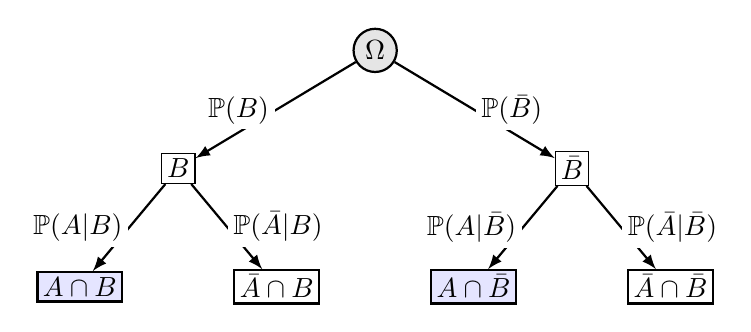
\begin{tikzpicture}[
  level 1/.style={sibling distance=5cm},
  level 2/.style={sibling distance=2.5cm},
  edge from parent/.style={draw,-latex, thick},
  every node/.style={align=center, fill=white, inner sep=2pt}
]
\node[circle, draw, thick, fill=gray!20] (root) {$\W$}
  child {node[rectangle, draw] (B) {$B$}
    child {node[rectangle, draw, fill=blue!10] (A1) {$A \cap B$}
        edge from parent node[left, pos=0.5] {$\Prob(A|B)$}
    }
    child {node[rectangle, draw] (Abar1) {$\bar{A} \cap B$}
        edge from parent node[right, pos=0.5] {$\Prob(\bar{A}|B)$}
    }
    edge from parent node[left, pos=0.5] {$\Prob(B)$}
  }
  child {node[rectangle, draw] (Bbar) {$\bar{B}$}
    child {node[rectangle, draw, fill=blue!10] (A2) {$A \cap \bar{B}$}
        edge from parent node[left, pos=0.5] {$\Prob(A|\bar{B})$}
    }
    child {node[rectangle, draw] (Abar2) {$\bar{A} \cap \bar{B}$}
        edge from parent node[right, pos=0.5] {$\Prob(\bar{A}|\bar{B})$}
    }
    edge from parent node[right, pos=0.5] {$\Prob(\bar{B})$}
  };
\end{tikzpicture}
\end{center}
\vspace{0.5cm}

\subsection{Heuristics \& Common Pitfalls}
\begin{itemize}
    \item \textbf{Pitfall: Confusing "Mutually Exclusive" with "Independent".} Mutually exclusive means $A \cap B = \emptyset$ (if one happens, the other strictly cannot). Independent means knowledge of one gives no information about the other. Non-empty mutually exclusive events are \textit{always} heavily dependent!
    \item \textbf{Fallacy: Base Rate Neglect.} When testing for a rare condition (e.g., $1\%$ prevalence), a test with $90\%$ accuracy does \textit{not} mean a positive result yields a $90\%$ chance of having the condition. Always adjust against the prior probability space $\Prob(D)$.
    \item \textbf{Heuristic: "At least one" $\to$ Complements.} Anytime a question asks for "at least one," compute $1 - \Prob(\text{none})$. This simplifies massive union calculations into simple intersection computations.
\end{itemize}

\newpage

% ==========================================
% PART 5: Conceptual Synthesis
% ==========================================
\section{Part 5: Conceptual Synthesis and The "Big Picture"}

\subsection{A) Thematic Connections: Sets to Measures}
The central theme of this chapter is the formal mapping between logical, set-theoretic structures and quantitative probability measures. Before this chapter, "probability" was merely counting favorable outcomes over total outcomes. Now, probability is formalized as a function $\Prob: \F \to [0,1]$ that takes abstract sets (events) as inputs. The laws of Boolean algebra (unions, intersections, complements) rigorously dictate the algebraic manipulation of these numerical measures. For example, De Morgan's laws acting on subsets identically map to rules like $1 - \Prob(A \cap B)$. 

\subsection{B) Forward Links: The Bedrock of Advanced Math}
The transition from events ($A, B \in \F$) to numerical mappings (Random Variables $Y: \W \to \R$) introduced at the end of the homework represents the most critical conceptual leap in modern statistics. By mapping abstract sample spaces to the real line $\R$, we set the foundation for the Lebesgue integral and cumulative distribution functions.
Furthermore, understanding partitions and conditional probability $\Prob(A|B)$ is the direct precursor to \textbf{Filtrations} ($\F_t$) and \textbf{Conditional Expectations} ($\E[X | \F_t]$), which form the rigorous mathematical foundation of Stochastic Calculus, Martingales, and dynamic modeling in continuous time.

\newpage

% ==========================================
% PART 6: Abstract Real-World Modeling
% ==========================================
\section{Part 6: Abstract Real-World Modeling (AI, ML, \& Quant Finance)}

\subsection{A) Concrete Scenarios}
The discrete Bayesian partitioning developed in Example 14 forms the direct mathematical skeleton for several advanced applications:
\begin{enumerate}
    \item \textbf{Machine Learning (Hidden Markov Models):} In Natural Language Processing and speech recognition, the observable text/audio is treated as an emission $A$, while the true grammatical tag or word is a hidden state partition $B_i$. We use Bayes' rule iteratively to find $\arg\max_i \Prob(B_i | A)$.
    \item \textbf{Quantitative Finance (Regime-Switching Models):} Market environments oscillate between "Bull" and "Bear" regimes, which are unobservable directly but emit varying volatility signatures. Quants use conditional probabilities to compute the posterior probability of being in a specific regime given a sequence of daily returns, continuously updating their prior via Bayes' rule.
\end{enumerate}

\subsection{B) Rigorous Model Setup: Regime-Switching Pricing Dynamics}
\textit{Let us abstract the concepts of this chapter into a quantitative finance model framing.}
Consider a probability space $(\W, \F, \Prob)$ representing infinite trajectories of an asset price process $\{S_t\}_{t=0}^\infty$.
We define an unobservable state space process $\{Z_t\}_{t=0}^\infty$ where $Z_t \in \{1, 2\}$, representing "Low Volatility" and "High Volatility" regimes. Let the initial prior partition be $\Prob(Z_0 = 1) = \pi_1$ and $\Prob(Z_0 = 2) = \pi_2$.

The observable market returns at time $t$ are $R_t = \log(S_t/S_{t-1})$. The conditional distribution of $R_t$ depends exclusively on the state $Z_t$. Assume $R_t | (Z_t = k) \sim \mathcal{N}(\mu_k, \sigma_k^2)$.
By extending the Law of Total Probability (Theorem \ref{thm:ltp}) to continuous densities, the unconditional density of the return is a Gaussian mixture:
\[ f(R_t) = \sum_{k=1}^2 f(R_t | Z_t = k)\Prob(Z_t = k) \]

In algorithmic trading, the true goal is to compute the posterior filtration of the hidden state given the history of returns $\F_t^R = \sigma(R_1, \dots, R_t)$. Utilizing a recursive extension of Bayes' Rule, the quantitative model updates the posterior state probabilities as follows:
\[ \Prob(Z_t = k | \F_t^R) = \frac{f(R_t | Z_t = k) \Prob(Z_t = k | \F_{t-1}^R)}{\sum_{j=1}^2 f(R_t | Z_t = j) \Prob(Z_t = j | \F_{t-1}^R)} \]
This dynamic Bayesian updating framework strictly relies on the axioms of conditional probability and partitions verified in your homework, operating natively within the $\sigma$-algebra generated by market observations.

\newpage

% ==========================================
% PART 7: Variations and Untested Concepts
% ==========================================
\section{Part 7: Common Variations and Untested Concepts}

A standard university curriculum in advanced probability theory introduces an additional, highly counter-intuitive nuance not explicitly covered in the provided PDF: \textbf{Conditional Independence}.

\begin{definition}[Conditional Independence]
Two events $A$ and $B$ are \textit{conditionally independent} given a third event $C$ (where $\Prob(C) > 0$) if:
\[ \Prob(A \cap B | C) = \Prob(A | C)\Prob(B | C) \]
\end{definition}

\textbf{Crucial Edge-Case Fact:} Independence does \textit{not} imply conditional independence, nor does conditional independence imply independence. The conditioning space inherently warps the measure.

\begin{proof}[Proof by Counterexample (Independent but not Conditionally Independent)]
Let two fair coins be tossed independently. Let $\W = \{HH, HT, TH, TT\}$, $\Prob(\{\omega\}) = 1/4$.
Let $A$ be the event that Coin 1 is Heads ($\{HH, HT\}$).
Let $B$ be the event that Coin 2 is Heads ($\{HH, TH\}$).
Clearly, $\Prob(A) = 1/2, \Prob(B) = 1/2$, and $\Prob(A \cap B) = \Prob(\{HH\}) = 1/4 = \Prob(A)\Prob(B)$. $A$ and $B$ are \textbf{independent}.

Now, define event $C$ as the event that \textit{exactly one} coin is Heads ($\{HT, TH\}$).
Conditioned on $C$, what is the measure of the space? $\Prob(C) = 1/2$.
Compute the conditionals:
$\Prob(A|C) = \frac{\Prob(A \cap C)}{\Prob(C)} = \frac{\Prob(\{HT\})}{1/2} = \frac{1/4}{1/2} = \frac{1}{2}$.
$\Prob(B|C) = \frac{\Prob(B \cap C)}{\Prob(C)} = \frac{\Prob(\{TH\})}{1/2} = \frac{1/4}{1/2} = \frac{1}{2}$.

If $A$ and $B$ were conditionally independent given $C$, then $\Prob(A \cap B | C)$ must equal $\Prob(A|C)\Prob(B|C) = (1/2)(1/2) = 1/4$.
However, observe the actual intersection: $\Prob(A \cap B \cap C) = \Prob(\{HH\} \cap \{HT, TH\}) = \Prob(\emptyset) = 0$.
Thus, $\Prob(A \cap B | C) = 0$. 
Since $0 \neq 1/4$, $A$ and $B$ are \textbf{not} conditionally independent given $C$.
\end{proof}
This nuance forms the mathematical basis for Explaining Away (Berkson's Paradox) in Bayesian Networks, a core ML concept.

\newpage

% ==========================================
% PART 8: Diagnostic Testing
% ==========================================
\section{Part 8: Advanced Diagnostic Testing: "Find the Flaw"}
Act as the grader. For each of the 5 problems below, a sophisticated proof or calculation is provided. Each contains exactly one subtle but critical mathematical or logical error. Find the flaw, explain it, and provide the correct logical step. \textit{(Solutions are available at the end of the document).}

\subsection*{Problem 1: Independence of Disjoint Sets}
\textbf{Question:} Let $\W$ be a sample space with events $A$ and $B$ such that $\Prob(A) = 0.4$ and $\Prob(B) = 0.5$. Suppose $A$ and $B$ cannot occur at the same time. Find the probability of their union, $\Prob(A \cup B)$.
\begin{proof}[Flawed Solution]
Since $A$ and $B$ cannot occur simultaneously, they are mutually exclusive. We want to find $\Prob(A \cup B)$. 
Using the additive law, $\Prob(A \cup B) = \Prob(A) + \Prob(B) - \Prob(A \cap B)$.
Since they are mutually exclusive, they are independent. 
Because they are independent, $\Prob(A \cap B) = \Prob(A)\Prob(B) = (0.4)(0.5) = 0.2$.
Therefore, $\Prob(A \cup B) = 0.4 + 0.5 - 0.2 = 0.7$.
\end{proof}

\subsection*{Problem 2: Conditional Additivity}
\textbf{Question:} Let $\Prob(A|B) = 0.3$ and $\Prob(A|C) = 0.5$. Given that $B$ and $C$ are mutually exclusive, what is $\Prob(A | B \cup C)$?
\begin{proof}[Flawed Solution]
Since $B$ and $C$ are mutually exclusive, $B \cap C = \emptyset$. We are asked to evaluate the probability of $A$ conditioned on the union of disjoint events. By the additivity of probabilities across disjoint conditioning events, we can distribute the conditional parameter:
$\Prob(A | B \cup C) = \Prob(A|B) + \Prob(A|C) = 0.3 + 0.5 = 0.8$.
\end{proof}

\subsection*{Problem 3: The Complement of the Conditional}
\textbf{Question:} An urn contains red and blue marbles. Let $A$ be the event of drawing a red marble on the second draw, and let $B$ be the event of drawing a blue marble on the first draw. If $\Prob(A|B) = 0.6$, find the probability of \textit{not} drawing a red marble on the second draw given that a blue marble was drawn first, i.e., $\Prob(\bar{A}|B)$.
\begin{proof}[Flawed Solution]
We know the total probability of an event and its complement must sum to 1.
Therefore, by the law of complements applied to conditionals, $\Prob(\bar{A}|B) = 1 - \Prob(A|\bar{B})$.
To proceed, we would need the value of $\Prob(A|\bar{B})$. Without this value, the problem cannot be solved.
\end{proof}

\subsection*{Problem 4: Transitivity of Independence}
\textbf{Question:} Suppose event $A$ is independent of event $B$, and event $B$ is independent of event $C$. Are events $A$ and $C$ independent?
\begin{proof}[Flawed Solution]
Assume $\Prob(A \cap B) = \Prob(A)\Prob(B)$ and $\Prob(B \cap C) = \Prob(B)\Prob(C)$.
To check if $A$ and $C$ are independent, consider the joint intersection:
$\Prob(A \cap C) = \Prob(A \cap (B \cup \bar{B}) \cap C) = \Prob(A \cap B \cap C) + \Prob(A \cap \bar{B} \cap C)$.
Since $B$ acts as an independent bridge mapping the sample space $\W$ transitively between mutually independent components, $A$ inherits independence from $C$. Thus, $\Prob(A \cap C) = \Prob(A)\Prob(C)$, so yes, they are independent.
\end{proof}

\subsection*{Problem 5: Extreme Conditioning}
\textbf{Question:} Let $X$ be a random variable representing the exact weight of a randomly chosen apple in grams, measured with infinite precision (continuous state space). Let $A$ be the event that the apple is perfectly red. What is the probability the apple is perfectly red given it weighs exactly $150.000...$ grams?
\begin{proof}[Flawed Solution]
We apply the strict definition of conditional probability derived from Kolmogorov's axioms:
\[ \Prob(A | X = 150) = \frac{\Prob(A \cap \{X=150\})}{\Prob(X=150)} \]
By evaluating the numerator and dividing by the denominator, we derive the posterior probability of the apple being red.
\end{proof}

% --- Solutions ---
\newpage
\subsection*{Solution Key for "Find the Flaw"}
\textbf{1. Independence of Disjoint Sets:}
\textit{Flaw:} "Since they are mutually exclusive, they are independent."
\textit{Resolution:} This is the most common logical fallacy in introductory probability. Mutually exclusive non-empty sets are \textit{never} independent. If $A$ happens, $B$ cannot happen, meaning knowledge of $A$ perfectly dictates $B$. Correct step: Since mutually exclusive, $\Prob(A \cap B) = 0$. Thus $\Prob(A \cup B) = 0.4 + 0.5 - 0 = 0.9$.

\textbf{2. Conditional Additivity:}
\textit{Flaw:} "additivity of probabilities across disjoint conditioning events... $\Prob(A | B \cup C) = \Prob(A|B) + \Prob(A|C)$"
\textit{Resolution:} Conditional probability distributes over unions in the \textit{numerator} (the event), not the denominator (the condition). In fact, $\Prob(A | B \cup C) = \frac{\Prob(A \cap B) + \Prob(A \cap C)}{\Prob(B) + \Prob(C)}$. It requires priors $\Prob(B)$ and $\Prob(C)$ to calculate as it is a weighted average of $\Prob(A|B)$ and $\Prob(A|C)$, guaranteeing the answer is between $0.3$ and $0.5$. Adding them to get $0.8$ is a gross violation of measure theory.

\textbf{3. The Complement of the Conditional:}
\textit{Flaw:} "$\Prob(\bar{A}|B) = 1 - \Prob(A|\bar{B})$"
\textit{Resolution:} The complement rule applies \textit{only} to the event being measured, not the condition space. The conditioning set limits the universe $\W$ to $B$. Within this new universe $B$, the axioms of probability remain identical. Thus, $\Prob(\bar{A}|B) = 1 - \Prob(A|B) = 1 - 0.6 = 0.4$. The problem is entirely solvable.

\textbf{4. Transitivity of Independence:}
\textit{Flaw:} "$B$ acts as an independent bridge... mapping... transitively."
\textit{Resolution:} Independence is \textit{not} a transitive mathematical relation. Consider rolling a die. Let $A = \{1, 2\}$, $B = \{2, 3, 4\}$, $C = \{1, 3, 5\}$. With $\Prob(\{\omega\}) = 1/6$, check independence: $\Prob(A \cap B) = 1/6 = \Prob(A)\Prob(B) = (1/3)(1/2)$. $A$ and $B$ are independent. Similarly, $\Prob(B \cap C) = 1/6 = \Prob(B)\Prob(C) = (1/2)(1/3)$. $B$ and $C$ are independent. However, $\Prob(A \cap C) = \Prob(\{1\}) = 1/6 \neq \Prob(A)\Prob(C) = 1/9$. $A$ and $C$ are absolutely not independent.

\textbf{5. Extreme Conditioning:}
\textit{Flaw:} "$\frac{\Prob(A \cap \{X=150\})}{\Prob(X=150)}$"
\textit{Resolution:} This involves a subtle but fatal measure-theoretic flaw known in the context of the Borel-Kolmogorov paradox. Because $X$ is continuous, the probability of taking on any exact point value is zero. Thus, $\Prob(X=150) = 0$. The definition of conditional probability $\Prob(A|B) = \Prob(A \cap B)/\Prob(B)$ strictly requires $\Prob(B) > 0$. Conditioning on a measure-zero set is undefined under elementary axioms and requires limit definitions via regular conditional probabilities using density functions or Radon-Nikodym derivatives.

\end{document}